\documentclass{beamer}
\usetheme[pageofpages=z,
          bullet=circle,
          titleline=true,
          alternativetitlepage=true,
          titlepagelogo=uplogo,
          ]{UVT}

\usepackage[utf8x]{inputenc}
\usepackage{czech}
\usepackage{minted}
\usepackage{graphicx}
% \usepackage{url}


\newenvironment{itemizex}%
  {\large \begin{itemize}%
    \setlength{\itemsep}{8pt}%
    \setlength{\parskip}{8pt}}%
  {\end{itemize}}

\newenvironment{enumeratex}%
  {\large \begin{enumerate}%
    \setlength{\itemsep}{6pt}%
    \setlength{\parskip}{6pt}}%
  {\end{enumerate}}

\newenvironment{itemizey}%
  {\large \begin{itemize}%
    \setlength{\itemsep}{6pt}%
    \setlength{\parskip}{6pt}}%
  {\end{itemize}}


\title{Základy programování 2 (KMI/ZP2 a KMI/UP2)}
\subtitle{Cvičení 7: Celková koncepce programu}
\author{Lukáš Havrlant}
\date{26. března 2013}
\institute{Univerzita Palackého}

\begin{document}

\begin{frame}[t,plain]
\titlepage
\end{frame}



\begin{frame}[t,fragile]\frametitle{Návratová hodnota funkce \texttt{main}} 
    \begin{itemizex}
        \item Již víme, že \texttt{main} je funkce.
        \item Tuto funkci volá operační systém po spuštění programu. 
        \item I tato funkce může vracet hodnotu -- typu \texttt{int}.
        \item Tuto návratovou hodnotu si \uv{vyzvedne} operační systém.
        \item Způsob zpracování není specifikován.
        \item Typicky se používá na oznamování chyb -- \texttt{return 0;} je vše v pořádku, \texttt{return 84;} může značit, že nastala chyba číslo 84.
    \end{itemizex}
\end{frame}


\begin{frame}[t,fragile]\frametitle{Parametry funkce \texttt{main}} 
    \begin{itemizex}
        \item Funkce \texttt{main} může mít žádný, nebo dva formální parametry.
        \item Z historických důvodů se jmenují \texttt{argc} (\uv{argument count}) a \texttt{argv} (\uv{argument vector}) a definují se takto:
\begin{minted}[linenos=true]{c} 
int main(int argc, char* argv[]);
\end{minted}
        \item Tyto argumenty předá operační systém, my je můžeme specifikovat v příkazové řádce:
\begin{minted}[linenos=true]{bash} 
./program.exe -c 10 "text s mezerou"
\end{minted}
        \item Do \texttt{argc} se uloží počet předaných argumentů, do \texttt{argv} se uloží jejich hodnoty.
    \end{itemizex}
\end{frame}


\begin{frame}[t,fragile]\frametitle{Parametry funkce \texttt{main} podruhé} 
\begin{minted}[linenos=true]{bash} 
./program.exe -c 10 "text s mezerou"
\end{minted}
    \begin{itemize}
        \item Hodnota \texttt{argc} bude rovna 4 -- počet předaných argumentů včetně názvu programu. 
        \item V \texttt{argv} bude uloženo:
\begin{minted}[linenos=true]{c} 
argv[0] = "./program.exe";
argv[1] = "-c";
argv[2] = "10";
argv[3] = "text s mezerou";
\end{minted}
        \item Na prvním místě je uložen název programu. Ostatní argumenty jsou odděleny mezerou. Pokud chceme mezeru jako součást argumentu, přidáme uvozovky.
    \end{itemize}
\end{frame}


\begin{frame}[t,fragile]\frametitle{Čísla se předávají jako řetězce} 
    \begin{itemizex}
        \item Pozor na to, že i čísla se předávají jako řetězec.
        \item Pokud chceme použít číslo opravdu jako číslo, je nutné ho zkonvertovat pomocí funkcí \texttt{atoi} (\uv{array to integer}) a \texttt{atof} (\uv{array to float}). Jsou v knihovně \texttt{stdlib.h}. Deklarace funkcí:
        \begin{minted}[linenos=true]{c} 
double atof (const char* str);
int atoi (const char* str);
        \end{minted}
        \item Příklad použití:
\begin{minted}[linenos=true]{c} 
int cislo = atoi("245") + atoi("55"); // 300
double des = atof("245.47") - atof("0.47"); // 245
\end{minted}
    \end{itemizex}
\end{frame}



\begin{frame}[t,fragile]\frametitle{Koncepce programu} 
    \begin{itemizex}
        \item Zatím jsem vytvářeli jeden program v jednom souboru, což je nepraktické a zlé. 
        \item V praxi dělíme různé části programu do samostatných souborů.
        \item V podstatě už to znáte: v knihovně \texttt{stdio} jsou funkce pro vstup/výstup, v \texttt{string} jsou funkce pro práci se s stringy atp.
        \item Otázka zní, jakým způsobem můžeme my vytvářet podobné knihovny? 
    \end{itemizex}
\end{frame}


\begin{frame}[t,fragile]\frametitle{Rozdělení do dvou souborů: příklad} 
\begin{itemizey}
    \item Mějme soubor funkce.c:
\begin{minted}[linenos=true]{c} 
int soucet(int a, int b) {
    return a + b;
}
\end{minted}
    \item A soubor hlavni.c:
\begin{minted}[linenos=true]{c} 
#include <stdio.h>
int main() {
    printf("2+3=%i\n", soucet(2, 3));
    return 0;
}
\end{minted}
    \item Jak zařídit, aby to fungovalo?
\end{itemizey}
\end{frame}


\begin{frame}[t,fragile]\frametitle{Direktiva \texttt{include}} 
    \begin{itemizex}
        \item \texttt{include} je preprocesorová direktiva, která přečte cílový soubor a jeho obsah vloží na místo, odkud jsme \texttt{include} volali.
        \item Tj. mohli bychom v souboru \texttt{hlavni.c} udělat toto:
\begin{minted}[linenos=true]{c} 
#include <stdio.h>
#include "funkce.c"
int main() {
    printf("2+3=%i\n", soucet(2, 3));
    return 0;
}
\end{minted}
        \item Obsah souboru \texttt{funkce.c} by se vložil na místo řádku s \texttt{\#include "funkce.c"}
    \end{itemizex}
\end{frame}


\begin{frame}[t,fragile]\frametitle{Nesprávně použitý \texttt{include}} 
Dostali bychom přibližně takový soubor: (ještě by se měl správně nahradit ten první \texttt{include})
\begin{minted}[linenos=true]{c} 
#include <stdio.h>
int soucet(int a, int b) {
    return a + b;
}
int main() {
    printf("2+3=%i\n", soucet(2, 3));
    return 0;
}
\end{minted}
Toto je ale \textbf{špatné řešení!} Chceme docítil odděleného překladu -- abychom byli schopni upravit soubor \texttt{funkce.c}, aniž bychom museli nutně přeložit soubor \texttt{hlavni.c}.
\end{frame}


\begin{frame}[t,fragile]\frametitle{Hlavičkový soubor} 
\begin{itemizey}
    \item Používáme namísto toho hlavičkové \texttt{.h} soubory. 
    \item Vytvoříme soubor \texttt{funkce.h}, do kterého vložíme deklarace funkcí, které jsou v souboru \texttt{funkce.c}, které chceme použít:

\begin{minted}[linenos=true]{c} 
int soucet(int, int);
\end{minted}
    \item V souboru \texttt{hlavni.c} vložíme pouze tento hlavičkový soubor. 
    \item Použítím hlavičkového souboru říkáme překladači: hele, v souboru \texttt{hlavni.c} budou možná použity ty a ty funkce, které jsou takového a makového typu. Později dodám jejich definice, s tím si zatím nelam hlavu. 
\end{itemizey}
\end{frame}


\begin{frame}[t,fragile]\frametitle{Deklarace funkce: opakování} 
    \begin{itemizex}
        \item Máme definici/implementaci nějaké funkce, např.:
\begin{minted}[linenos=true]{c} 
double prumer(double* cisla, int pocet) { 
    /* implementace */ 
}
\end{minted}
        \item Deklarace takové funkce je pak ořezaná hlavička funkce -- obsahuje návratový typ, název a parametry. Nemusíte uvádět názvy parametrů:
\begin{minted}[linenos=true]{c} 
double prumer(double*, int);
\end{minted}
    \end{itemizex}
\end{frame}


\begin{frame}[t,fragile]\frametitle{Jak budou nyní vypadat naše tři soubory?} 
hlavni.c:
\begin{minted}[linenos=true]{c} 
#include <stdio.h>
#include "funkce.h"
int main() {
    printf("2+3=%i\n", soucet(2, 3));
    return 0;
}
\end{minted}
funkce.c: (obsahuje definice funkcí)
\begin{minted}[linenos=true]{c} 
int soucet(int a, int b) {
    return a + b;
}
\end{minted}
funkce.h: (obsahuje deklarace funkcí, které jsou v \texttt{funkce.c})
\begin{minted}[linenos=true]{c} 
int soucet(int, int);
\end{minted}
\end{frame}


\begin{frame}[t,fragile]\frametitle{Hlavičkové soubory: rekapitulace} 
    \begin{itemizex}
        \item Hlavičkový soubor má typicky stejné jméno jako \texttt{.c} soubor, liší se jen příponou: \texttt{hlavni.c} a \texttt{hlavni.h}
        \item Hlavičkový soubor \texttt{hlavni.h} obsahuje deklarace funkcí, které chceme ze souboru \texttt{hlavni.c} sdílet.
        \item Pokud chceme v souboru \texttt{hlavni.c} používat funkce ze souboru \texttt{vypocty.c}, vložíme do souboru \texttt{hlavni.c} hlavičkový soubor \texttt{vypocty.h}.
        % \item Pokud máme v souboru \texttt{vypocty.c} nějakou pomocnou funkci a nechceme, aby ji mohl používat soubor \texttt{hlavni.c}, nevložíme deklaraci funkce do hlavičkového souboru.
    \end{itemizex}
\end{frame}


\begin{frame}[t,fragile]\frametitle{Jak zabránit vícenásobnému vložení} 
    \begin{itemize}
        \item Může se stát, že dva různé soubory vkládají jednu a tutéž knihovnu, což je obecně nežádoucí.
        \item K zabránění druhého vložení můžeme použít fígl s \texttt{\#ifndef} v hlavičkovém souboru. Můžeme modifikovat soubor \texttt{funkce.h}:
\begin{minted}[linenos=true]{c} 
#ifndef FUNKCE_H
#define FUNKCE_H
int soucet(int, int);
#endif
\end{minted}
        \item Pokud není definovaná konstanta FUNKCE\_H, tak se definuje a následují deklarace.
        \item Pokud konstanta je definovaná, preprocesor celý obsah až po \texttt{\#endif} smaže. 
    \end{itemize}
\end{frame}


\begin{frame}[t,fragile]\frametitle{Oddělený překlad pomocí objektových souborů} 
\begin{figure}[htb]
    \centering
    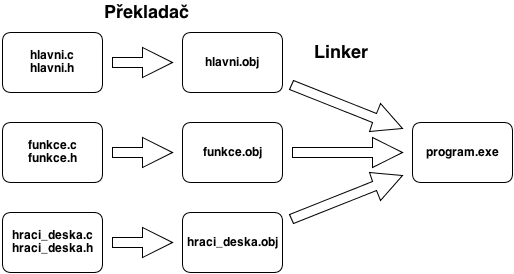
\includegraphics[scale=0.6]{img/schema.pdf}
    \caption{Zjednodušené schéma překladu programu}
\end{figure}
\end{frame}


\begin{frame}[t,fragile]\frametitle{Objektový soubor} 
    \begin{itemizex}
        \item Objektový soubor představuje zkompilovaný \texttt{.c} soubor. 
        \item Pokud změníme funkci v souboru \texttt{funkce.c}, můžeme jen přeložit tento soubor, zavolat linker a ten znovu spojí \texttt{.obj} soubory.
        \item Soubor \texttt{hlavni.obj} se nemusí změnit, tj. \texttt{hlavni.c} se nemusí překládat. 
        \item Jinými slovy: můžeme měnit kód souboru \texttt{hlavni.c} bez toho, aniž bychom měli přístup k \texttt{funkce.c}. Stačí nám výsledný \texttt{.obj} soubor.
    \end{itemizex}
\end{frame}


\begin{frame}[t,fragile]\frametitle{Oddělený překlad prakticky} 
    \begin{itemizex}
        \item Vývojová prostředí to obvykle dělají automaticky. Stačí vytvořit požadované \texttt{.c} a \texttt{.h} soubory a kliknout na magické tlačítko (\uv{Compile}, \uv{Build} atp.)
    \end{itemizex}
\end{frame}


\begin{frame}[t,fragile]\frametitle{Oddělený překlad v příkazovém řádku} 
    \begin{itemizex}
        \item V příkazové řádce např. pomocí překladače \texttt{gcc} takto (objektové soubory zde získají příponu \texttt{.o} místo \texttt{.obj}):
\begin{minted}[linenos=true]{bash} 
$ gcc -c hlavni.c
$ gcc -c funkce.c
$ gcc hlavni.o funkce.o -o program
$ ./program
2+3=5
\end{minted}
        \item Případně bez mezikroku: 
\begin{minted}[linenos=true]{bash} 
$ gcc funkce.c hlavni.c -o program
$ ./program
2+3=5
\end{minted}
    \end{itemizex}
\end{frame}


\begin{frame}[t,fragile]\frametitle{Poznámky na konec} 
    \begin{itemize}
        \item \texttt{\#include <nazev>} hledá knihovnu v systémovém adresáři, \texttt{\#include "nazev"} hledá knihovnu relativně vůči souboru.
        \item V hlavičkovém souboru nemusí být pomocné funkce a obecně funkce, které nechceme sdílet. 
        \item V hlavičkovém souboru mohou být i další věci -- typy definované přes \texttt{typedef}, které chceme veřejně sdílet, konstanty apod. 
        \item Pokud např. \texttt{vypocet.c} pracuje s typem \texttt{zlomek} a my tento typ chceme použít i v souboru \texttt{hlavni.c}, musí být typ zlomek definován už v \texttt{vypocet.h}.
        \item Samotný soubor \texttt{vypocet.c} může includnout svůj hlavičkový soubor. 
    \end{itemize}
\end{frame}


\begin{frame}[t,fragile]{Úlohy}
\begin{center}
\vskip 1cm
{\Large Seznam úloh je na \url{http://KMIzp2.jdem.cz/}}
\vskip 2cm
\url{http://tux.inf.upol.cz/~havrlant/}
\end{center}
\end{frame}


\end{document}